\documentclass[10pt, a4paper]{article}
\usepackage[utf8]{inputenc}
\usepackage[T1]{fontenc,url}
\usepackage{multicol}
\usepackage{multirow}
\usepackage{parskip}
\usepackage{lmodern}
\usepackage{microtype}
\usepackage{verbatim}
\usepackage{amsmath, amssymb}
\usepackage{tikz}
\usepackage{physics}
\usepackage{mathtools}
\usepackage{algorithm}
\usepackage{algpseudocode}
\usepackage{listings}
\usepackage{enumerate}
\usepackage{graphicx}
\usepackage{float}
\usepackage{hyperref}
\usepackage{tabularx}
\usepackage{siunitx}
\usepackage{fancyvrb}
%\usepackage{natbib}
%\bibliographystyle{dinat}
\usepackage[makeroom]{cancel}
\usepackage[margin=2.0cm]{geometry}
\usepackage{pdfpages}
\usepackage[margin=10pt, textfont={small, it}, labelfont={bf}, labelsep=endash]{caption}
\renewcommand{\baselinestretch}{1}

\begin{document}
\title{COMAP - Compression of level 1 files}
\author{
    \begin{tabular}{r l}
        Jonas Gahr Sturtzel Lunde & (\texttt{jonassl@astro.uio.no})
    \end{tabular}}
% \date{}    % if commented out, the date is set to the current date
\maketitle
Relevant code found at \url{https://github.com/jgslunde/comap_compress}
\vspace{0.7cm}

\section*{Summary}
Compression of a 50-60GB 1 hour obervation, using the suggested GZIP level 3 compression:
\begin{itemize}
    \item Compression time: $\sim$ 70 minutes
    \item Compression ratio: $\sim$ 2.45
    \item Decompression time: $\sim$ 3 minutes
\end{itemize}

The hdf5 library contains support for compressing datasets, which we can use to reduce the storage requirements of our level 1 files. A typical level 1 file, consisting of a 1 hour obervation, is of the size 50-60GB, which can be reduced by a factor of around 2.4 through lossless compression. The compression takes somewhat over an hour to perform on a typical processor core. The compression itself is not parallelizable, but multiple compressions can be run in parallel. Once compressed, the hdf5 files function as normal, and will be automatically decompressed once read. The decompression typically takes 3 minutes per file.


\section*{Implementation}
The compression can be done with the h5repack command:

\texttt{h5repack -f /spectrometer/tod:SHUF -f /spectrometer/tod:GZIP=3\\
-l /spectrometer/tod:CHUNK=1x4x1024x4000 oldfile.hd5 newfile.hd5}

We can specify that only parts of the hdf5 hierarchy be compressed, as done above with \texttt{/spectrometer/tod}. We do this because over $99\%$ of the data is in this single data field, making compression of other quantities meaningless. We can also specify a level of GZIP compression in the range 1-9, where we have in the above example selected 3.

\section{Chunking}
The \texttt{-l /spectrometer/tod:CHUNK=1x4x1024x4000} part of the repack command specifies the compression chunking. Chunks are the parts of the data which are compressed together, such that all data of a chunk must be decompressed in order to access any of it. Bigger chunks typically give better compression, while smaller chunks allow for more fine-grained decompression. Our data is typically of dimensions 20x4x1024x200000 (feed, sideband, frequency, time). As we often wish to decompress a single scan within an obsid (typically 20,000 of the total 200,000 TOD points), chunks of 1x4x1024x4000 hits a sweet-spot of both good compression levels, and the ability to decompress chunks of only 4,000 TOD points.


\section*{Compression}
hdf5 ships with only a handful of compression types, of which GZIP is the most efficient. There exists more effective compression algorithms, but for our purposes, it's important that our implementation is supported by out of the box hdf5.

hdf5 also comes with a shuffle filter (\texttt{-f /spectrometer/tod:SHUF}), which reorders the data for more efficient compression. We always enable this.

GZIP offers compression levels in the range of 1-9. The figures below show its impact on compression ratio, compression time, and decompression time. GZIP levels above 7 are not shown, as the compression times of these levels were ridiculous, without meaningful gain in other areas.

My suggestion, based on these results, is to employ the level 3 GZIP compression, which seems to be very well suited for our needs. The only real contenter is level 4, which offers the best compression, ~1\% above that of level 3, but at a cost of a ~25\% increase in decompression time, which is important to us.

\begin{figure}[H]
    \centering
    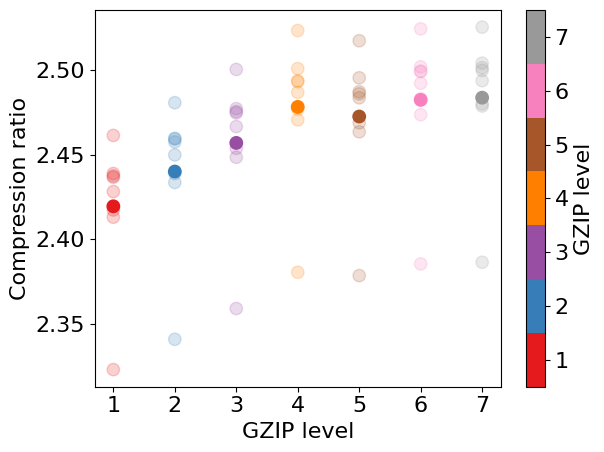
\includegraphics[scale=0.55]{plots/gzip_compratio.png}
    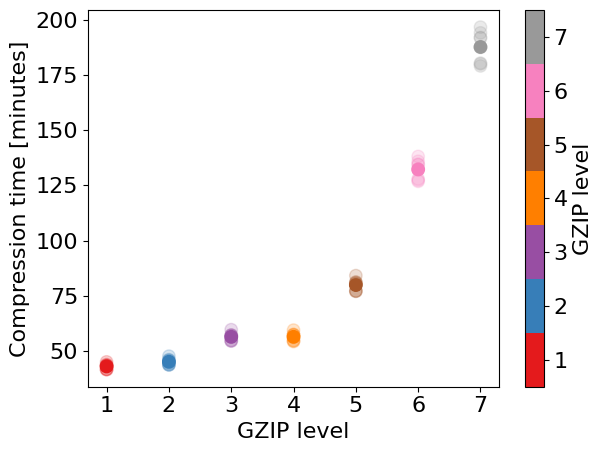
\includegraphics[scale=0.55]{plots/gzip_comptime.png}
    \caption{Compression ratio (left) and compression time (right) of 5 random 50-60GB observations, as function of GZIP level. The mean of the 5 points are shown as a solid dot.}
    \label{fig:fig1}
\end{figure}

\begin{figure}[H]
    \centering
    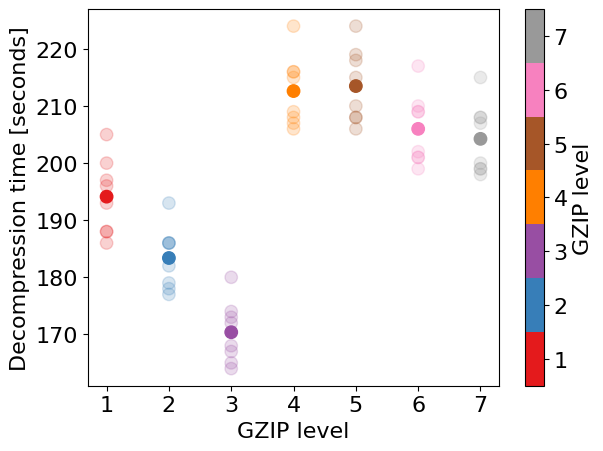
\includegraphics[scale=0.55]{plots/gzip_decomptime.png}
    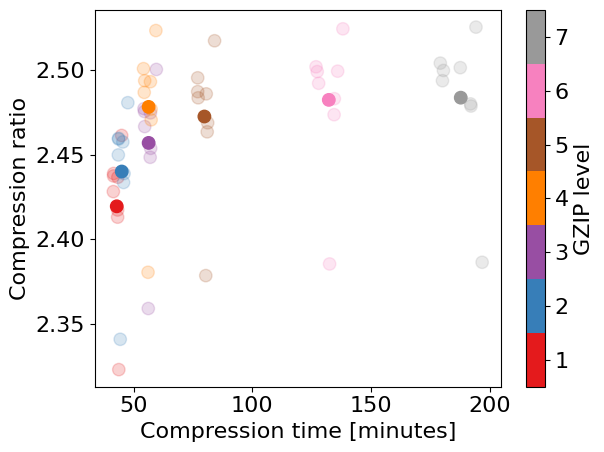
\includegraphics[scale=0.55]{plots/comptime_compratio.png}
    \caption{Decompression time as function of GZIP level (left), and relation between compression time and compression ratio (right) of 5 random 50-60GB observations. The mean of the 5 points are shown as a solid dot.}
    \label{}
\end{figure}


\section*{Parallel compression}
As the compression itself, on a single file, is not parallel, the only way to support parallel compression is to compress several files in parallel. However, GZIP has very low memory usage, and frequently reads and writes to disk. I ran into I/O bottlenecks when compressing many files in parallel. I've found no option in h5repack to increase the memory read/write buffer. My current solution involves reading files to a ram-disk before compression, which means a much larger memory usage.


\end{document}